\documentclass[11pt,aspectratio=169]{beamer}

% -------------------- THEME & LAYOUT --------------------
\usetheme{Madrid}
\usecolortheme{dolphin} % base color scheme
\usefonttheme{professionalfonts}
\setbeamercovered{transparent}
\setbeamertemplate{navigation symbols}{}   % remove navigation buttons
\setbeamertemplate{caption}[numbered]      % numbered captions
\setbeamertemplate{itemize items}[triangle]
\setbeamersize{text margin left=1.2cm,text margin right=1.2cm} % adjust to taste
% -------------------- GLOBAL FONT SETTINGS --------------------

% 1. Force the base beamer font to small
\setbeamerfont{normal text}{size=\small}

% 2. Force math environments to follow the "small" font size
\setbeamerfont{math text}{size=\small}
\setbeamerfont{equation}{size=\small}

% 3. Redefine \normalsize itself 
% This ensures equations and lists (which look for \normalsize) use  instead.
\let\oldnormalsize\normalsize
\renewcommand{\normalsize}{\oldnormalsize\small}

% 4. Ensure lists also stay small
\setbeamerfont{itemize/enumerate body}{size=\small}
\setbeamerfont{itemize/enumerate subbody}{size=\small}
% -------------------- FONTS & TYPOGRAPHY --------------------
\usepackage[T1]{fontenc}
\usepackage[utf8]{inputenc}
\usepackage{newpxtext,newpxmath} % Palatino-like font & math
\usepackage{microtype}

% -------------------- MATH, TABLES & GRAPHICS --------------------
\usepackage{amsmath,amssymb,amsfonts,mathtools}
\usepackage{bm,booktabs,siunitx,graphicx}
\graphicspath{{./}{./figures/}}
\renewcommand{\theequation}{14.\arabic{equation}}

% -------------------- UTILITIES --------------------
\usepackage{appendixnumberbeamer}
\usepackage{ragged2e}
\usepackage{xspace}
\usepackage{csquotes}
% -------------------- Bibliography --------------------
\usepackage[backend=biber,style=authoryear]{biblatex}
\addbibresource{sources.bib}
\usepackage{xcolor}

% -------------------- COLORS & EMPHASIS --------------------
\definecolor{myblue}{RGB}{0,70,140}
\definecolor{myred}{RGB}{180,30,30}
\definecolor{mygreen}{RGB}{0,120,70}
\definecolor{gold}{RGB}{184,134,11}

\setbeamercolor{title}{fg=gold}       % title page
\setbeamercolor{frametitle}{fg=gold}  % slide titles
\setbeamercolor{structure}{fg=gold}   % bullets, sections, links
\setbeamercolor{section in head/foot}{fg=gold,bg=black!10} % gold text on light background

% -------------------- FOOTLINE --------------------
\setbeamertemplate{footline}{
  \leavevmode%
  \hbox{%
    % Section links (hidden if no current section)
    \begin{beamercolorbox}[wd=0.7\paperwidth,ht=2.5ex,dp=1.5ex,leftskip=1.4em]{section in head/foot}%
      \ifx\insertsection\empty
        % nothing
      \else
        Section: \insertsection
      \fi
    \end{beamercolorbox}%
    % Frame number right
    \begin{beamercolorbox}[wd=0.3\paperwidth,ht=2.5ex,dp=1.5ex,leftskip=3.8cm]{section in head/foot}%
      \insertframenumber/\inserttotalframenumber
    \end{beamercolorbox}%
  }%
  \vskip1pt%
}



\newcommand{\highlight}[1]{\textcolor{myblue}{#1}}
\newcommand{\warning}[1]{\textcolor{myred}{#1}}

% -------------------- SHORTCUTS --------------------
\newcommand{\E}{\mathbb{E}}
\newcommand{\R}{\mathbb{R}}
\newcommand{\dd}{\mathrm{d}}
\newcommand{\mc}[1]{\mathcal{#1}}
\newcommand{\bb}[1]{\mathbb{#1}}
\newcommand{\uc}{U_c}
\newcommand{\zg}{Z_g}

% -------------------- TIGHTER DISPLAY MATH --------------------
\makeatletter
\g@addto@macro\normalsize{%
  \setlength\abovedisplayskip{8pt}%
  \setlength\belowdisplayskip{8pt}%
  \setlength\abovedisplayshortskip{6pt}%
  \setlength\belowdisplayshortskip{6pt}%
}
\makeatother
\setbeamertemplate{frametitle}{
  \nointerlineskip
  \begin{beamercolorbox}[wd=\paperwidth,ht=3.5ex,dp=1ex,center]{frametitle}
    \centering\insertframetitle
  \end{beamercolorbox}
}

% -------------------- SECTION ROADMAP --------------------
\AtBeginSection[]
{
  \begin{frame}
    \tableofcontents[currentsection, hideothersubsections]
  \end{frame}
}


\begin{document}
\setcounter{equation}{0}


% ===================== TITLE SLIDE =====================
\begin{frame}[plain] % 'plain' removes header/footer for the title slide

\begin{columns}[T,totalwidth=\textwidth]

% ----- Left column: Main title, professor, chapter -----
\begin{column}{0.45\textwidth}
\vspace{2cm}

% Main title
{\usebeamercolor[fg]{title}\LARGE\textbf{Monetary Economics}\\[0.3cm]
\LARGE\textbf{and Policy}} 

\vspace{0.5cm}

% Professor name and date
{\large\textit{Pierpaolo Benigno}}\\[0.1cm]

\vspace{1cm}

% Chapter and subtitle
{\usebeamercolor[fg]{frametitle}\large Chapter 14: The Future of Monetary Policy}

\end{column}

% ----- Right column: Image -----
\begin{column}{0.55\textwidth}
\vspace{1cm}
\centering
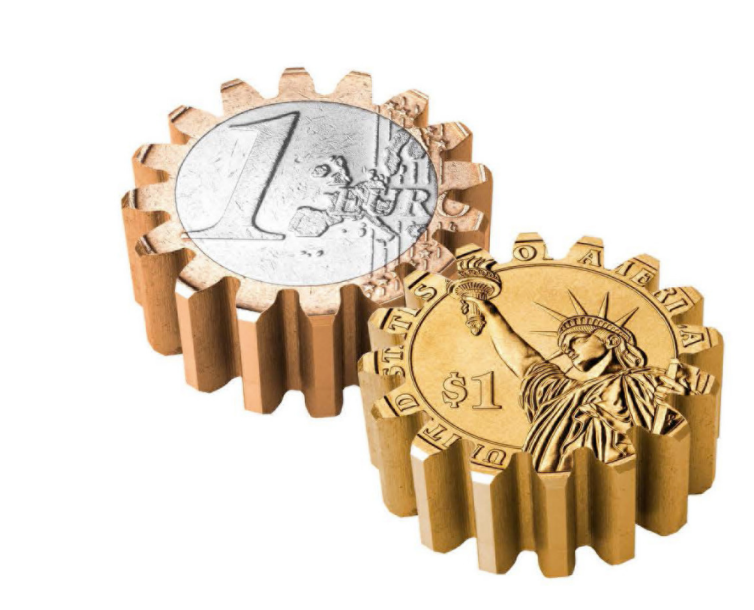
\includegraphics[width=0.9\linewidth]{Cover.png}
\end{column}

\end{columns}

% ----- Footer text (bottom-right corner) -----
\vspace*{2cm} % adjust if needed
\hfill{\large\textit{}}

\end{frame}

%-----------------------------------------------------------

% OUTLINE
\begin{frame}{Outline}
\tableofcontents
\end{frame}

%===========================================================
\section{A Benchmark: Neutrality and the ``Virtual Room''}
%===========================================================

\begin{frame}{A Stable Monetary Framework}
\small
\begin{itemize}
  \item The book highlights a complex governance of currency: value anchoring, liquidity provision, crisis management, and fiscal interactions.
  \item Because the same institution can stabilize some margins while distorting others, sweeping conclusions can lead to contradictions.
  \item Still, offering a unified framework in the book invites a preliminary \enquote{big-picture} discussion of the characteristics of a \textbf{stable monetary framework} (cf.\ \cite{friedman1960program}, \cite{friedmanschwartz1986}).
\end{itemize}
\end{frame}

\begin{frame}{From Barter to the Need for a Monetary System}
\small
\begin{itemize}
  \item Barter economies are limited by the \textbf{double coincidence of wants}.
  \vspace{1em}
  \item Exchange is confined to proximity and bilateral matching; economic development is constrained.
    \vspace{1em}
  \item A currency system and market economy can be interpreted as institutions that approximate a more complete coordination device than barter.
\end{itemize}
\end{frame}

\begin{frame}{Medieval Europe and ``Near-Barter'' Conditions}
\small
\begin{itemize}
  \item \textcite{cipolla1956}: In medieval Europe the demand for coins was depressed. Coins were only one of many means of settlement.
  \item Even debts stipulated in coin units were often settled with commodities (vases, cloths, horses).
  \item A central reason was an \textbf{inefficient market}:
  people could not rely on markets to have what they wanted (\cite{cipolla1956}).
  \item With weak market reliability, there is little incentive to hold coins for future transactions with third parties.
\end{itemize}
\end{frame}

\begin{frame}{The ``Virtual Room'' Benchmark}
\small
\begin{itemize}
  \item Imagine a hypothetical ``virtual room'' where all current and future generations reveal their plans.
  \item A virtual Walrasian auctioneer adjusts intratemporal and intertemporal prices so plans are mutually compatible.
  \item In that ideal benchmark, no currency is needed as an intermediary.
  \item The benchmark is useful because it highlights a desideratum:
  a currency should be as \textbf{neutral} as possible relative to the allocation that would obtain under full-information coordination.
\end{itemize}
\end{frame}

\begin{frame}{Currency Irrelevance as a Desideratum}
\small
\begin{itemize}
  \item If currency were ``irrelevant'' in the benchmark sense, it would not distort the compatible plans that solve the virtual-room problem.
  \item It is hard to imagine a world where a worthless currency improves everyone’s real plans:
  the benchmark suggests that distortions from currency manipulation are costs, not benefits.
  \item In a second-best world, a currency system and market economy may be the best approximation we can get to the virtual-room coordination device.
\end{itemize}
\end{frame}

%===========================================================
\section{History and the Temptation to Manipulate}
%===========================================================

\begin{frame}{The First Distortion: Granting Favored Status}
\small
\begin{itemize}
  \item Moving away from barter by selecting a commodity as a privileged medium of exchange creates a distortion:
  \begin{itemize}
    \item the privileged commodity gains purchasing power relative to the pre-currency allocation,
    \item agents holding more of it benefit disproportionately.
  \end{itemize}
  \item Even if it solves the coincidence-of-wants problem, it creates distributional consequences.
\end{itemize}
\end{frame}

\begin{frame}{Manipulation Under Metallic Coin Regimes}
\small
\begin{itemize}
  \item Historical practice under sovereign control of coinage:
  \begin{itemize}
    \item seigniorage extraction,
    \item debasement of intrinsic value,
    \item monopolistic management of issuance and verification.
  \end{itemize}
  \item These practices aimed at appropriating real resources and thus increased distortions.
\end{itemize}
\end{frame}

\begin{frame}{Inconvertible Paper Currency and Stronger Temptations}
\small
\begin{itemize}
  \item Under inconvertible paper currency, currency is ``what can be printed at will.''
  \item This heightens the temptation to manipulate real allocations through monetary expansion.
  \item Central banks historically emerged from urgent needs of the state:
  \begin{itemize}
    \item financing the state,
    \item averting banking liquidity crises.
  \end{itemize}
  \item These actions, one way or another, distort allocations in favor of the state and/or the banking sector.
\end{itemize}
\end{frame}

\begin{frame}{2007--2008 and COVID: Buyers of Last Resort}
\small
\begin{itemize}
  \item Recent history: central banks became buyers of last resort for ``almost everything'' during:
  \begin{itemize}
    \item the Global Financial Crisis (2007--2008),
    \item the COVID-19 pandemic.
  \end{itemize}
  \item Policymakers faced hard governance decisions; the sequence around Lehman highlights the difficulty:
  \begin{itemize}
    \item failure allowed on Sept.\ 15, 2008,
    \item immediate shift toward broad purchases the next day.
  \end{itemize}
  \item Whether such interventions represent ``appropriate'' money governance is debatable.
\end{itemize}
\end{frame}

\begin{frame}{Europe: A New Era of Central Bank Backing}
\small
\begin{itemize}
  \item The Euro Area illustrates evolving monetary--fiscal dynamics:
  \begin{itemize}
    \item ``whatever it takes'' (Draghi, July 26, 2012),
    \item pandemic-era shifts and large-scale national debt purchases.
  \end{itemize}
  \item These interventions loosened sustainability constraints and enabled large fiscal actions.
  \item The resulting allocation distortions have arguably been reflected in the post-COVID inflation surge.
\end{itemize}
\end{frame}

\begin{frame}{The Difficult Second-Best Reality}
\small
\begin{itemize}
  \item From the virtual-room benchmark perspective, achieving a neutral currency is challenging even in a second-best world.
  \item Citizens appear ``consigned'' to currency jurisdictions vulnerable to manipulation.
  \item This motivates interest in mechanisms that could discipline or replace national monopoly currency provision.
\end{itemize}
\end{frame}

%===========================================================
\section{Cryptocurrencies: Competition and Verification}
%===========================================================

\begin{frame}{Cryptocurrencies as a Watershed Event}
\small
\begin{itemize}
  \item The emergence of private digital currencies introduces:
  \begin{itemize}
    \item competition in currency adoption and usage,
    \item systems that transcend national borders,
    \item the possibility of switching currency systems without relocating.
  \end{itemize}
  \item This can be a powerful force for better currencies or at least meaningful choice.
\end{itemize}
\end{frame}

\begin{frame}{Historical Note: Currency Competition Is Not New}
\small
\begin{itemize}
  \item A single national currency is relatively recent.
  \item In metallic systems, competition among coins with different intrinsic content was common.
  \item Such competition often produced Gresham’s-law phenomena:
  ``good'' coins hoarded, ``bad'' coins circulate.
  \item Modern crypto competition differs by operating globally and digitally.
\end{itemize}
\end{frame}

\begin{frame}{Hayek: Denationalization and Competition as Discipline}
\small
\begin{itemize}
  \item \textcite{Hayek1976Denationalization}: competition could constrain issuers more effectively than redeemability obligations.
  \item He envisions dominance of a currency that maintains purchasing power (a ``real dollar'').
  \item Different commodity baskets relevant for different groups could imply coexistence of multiple currencies.
  \item A stable purchasing-power currency could also be attractive as protection against fiscal and financial dominance.
\end{itemize}
\end{frame}

\begin{frame}{\textcite{friedmanschwartz1986}: A Cautious View}
\small
\begin{itemize}
  \item \textcite{friedmanschwartz1986} take a cautious view: it is \textbf{not yet established} that private fiduciary currencies can reliably deliver both efficiency and safety without public authority or a well-defined institutional backstop.
  \item They therefore adopt an \textbf{agnostic} stance on the optimal monetary arrangement (public vs.\ private), emphasizing that the answer is ultimately empirical and institutional.
  \item Still, allowing \textbf{competition} in currency and payments can discipline government issuers: if public management performs poorly, market alternatives can constrain policy mistakes—consistent with their broader theme that \textbf{government failure} can be as severe as \textbf{market failure} in some circumstances.
\end{itemize}
\end{frame}

\begin{frame}{Cryptographic Verification: A Second Innovation}
\small
\begin{itemize}
  \item Cryptocurrencies bring a decentralized verification system based on cryptography.
  \item It grants no special privilege except for mathematical consensus.
  \item This shifts verification from third-party judgment and courts toward a ``cryptography guarantee''.
  \item It speaks to contract-enforcement and fraud-prevention difficulties emphasized by  \textcite{friedmanschwartz1986}.
\end{itemize}
\end{frame}

\begin{frame}{Smart Contracts and Decentralized Finance}
\small
\begin{itemize}
  \item Decentralized finance extends the idea via smart contracts:
  \begin{itemize}
    \item automated, rule-based execution,
    \item potentially reduced reliance on subjective enforcement.
  \end{itemize}
  \item This technological direction could improve the transparency of risk and the enforceability of promises-to-pay.
\end{itemize}
\end{frame}

%===========================================================
\section{Implications for the Future Design of Monetary Policy}
%===========================================================

\begin{frame}{What the Book Helps Us Organize}
\small
\begin{itemize}
  \item The book provides a framework to reason about:
  \begin{itemize}
    \item anchoring the value of an intrinsically worthless currency,
    \item supplying liquidity / safe assets,
    \item macroeconomic stabilization (inflation/output),
    \item crisis intervention and prevention.
  \end{itemize}
  \item These dimensions matter regardless of whether the dominant currency is public or private.
\end{itemize}
\end{frame}

\begin{frame}{Separation of Monetary and Fiscal Policy}
\small
\begin{itemize}
  \item Chapters 1, 2, and 13 provide arguments for separating monetary and fiscal policy.
  \item Giving special guarantees to treasury liabilities or direct deficit finance:
  \begin{itemize}
    \item makes currency value depend unnecessarily on fiscal policy,
    \item increases the risk of fiscal dominance and instability.
  \end{itemize}
  \item The logic is sharpened by a key insight: the currency does not even require fiscal backing to be anchored (under the principles developed earlier in the book).
\end{itemize}
\end{frame}

\begin{frame}{Backing Without the Treasury: Assets and Real Backing}
\small
\begin{itemize}
  \item If seigniorage is weakened by competition, value control hinges more on backing via assets.
  \item A central bank can support its liabilities by holding:
  \begin{itemize}
    \item high-quality default-free securities,
    \item and/or tangible real assets (e.g.\ gold).
  \end{itemize}
  \item Gold provides an immediate, simple anchor when a newly created currency lacks deep safe-asset markets.
  \item Historical note (\cite{cipolla1956}): early acceptance of new gold coins could be difficult, even when intrinsically valuable.
\end{itemize}
\end{frame}

\begin{frame}{Operational Framework: What to Target}
\small
\begin{itemize}
  \item Currency-value stability can be encoded as:
  \begin{itemize}
    \item inflation targeting,
    \item price-level targeting,
    \item nominal spending targeting.
  \end{itemize}
  \item A low positive inflation trend can be useful as a buffer against distortions highlighted in the book.
  \item Digitization may reduce the relevance of some distortions (e.g.\ the ZLB), though other distortions may become more important.
\end{itemize}
\end{frame}

\begin{frame}{Neutrality as the Issuer’s Responsibility}
\small
\begin{itemize}
  \item In a competitive environment, the issuer of the unit of account should:
  \begin{itemize}
    \item assume sole responsibility for stabilizing purchasing power,
    \item play a neutral role, avoiding distortions that favor particular groups.
  \end{itemize}
  \item This is the closest feasible approximation to the virtual-room benchmark in a second-best world.
\end{itemize}
\end{frame}

\begin{frame}{Who Should Supply Liquidity? Lessons from Chapters 4 and 11}
\small
\begin{itemize}
  \item Chapters 4 and 11 provide contrasting but complementary lessons.
  \item \textbf{Chapter 4 (frictionless private money creation):}
  \begin{itemize}
    \item competition can satisfy liquidity needs,
    \item private liquidity does not interfere with unit-of-account value control.
  \end{itemize}
  \item \textbf{Chapter 11 (frictions and pseudo-safe assets):}
  \begin{itemize}
    \item frictions can produce pseudo-safe liquidity and crises,
    \item poor private liquidity performance can cause contractions and disinflationary pressure,
    \item the issuer must substitute low-quality private liquidity with high-quality public liquidity in crises.
  \end{itemize}
\end{itemize}
\end{frame}

\begin{frame}{Public Liquidity, Backing, and Dominance Risks}
\small
\begin{itemize}
  \item One reading of Chapter 11: even beyond crises, the unit-of-account issuer may need to supply liquidity broadly.
  \item But abundant liquidity requires equivalent backing:
  \begin{itemize}
    \item either high-quality assets on the issuer’s balance sheet,
    \item or (if integrated with the treasury) current and future taxes.
  \end{itemize}
  \item Both routes create possible dominance risks:
  \begin{itemize}
    \item financial dominance through private-sector balance-sheet exposure,
    \item fiscal dominance through treasury linkage.
  \end{itemize}
\end{itemize}
\end{frame}

\begin{frame}{Why Private Money Creation Breaks Down}
\small
\begin{itemize}
  \item Chapter 11’s crisis mechanism stems from an underdeveloped intermediation process:
  \begin{itemize}
    \item opacity of intermediaries’ balance sheets (especially asset quality),
    \item limited ability to evaluate risk and liquidity characteristics correctly.
  \end{itemize}
  \item New technologies (cryptographic guarantees) could improve transparency and verification:
  \begin{itemize}
    \item better pricing of risk and liquidity,
    \item competition can then more reliably determine the amount of liquidity supplied.
  \end{itemize}
\end{itemize}
\end{frame}

\begin{frame}{Maturity Transformation as a Symptom of Underdevelopment}
\small
\begin{itemize}
  \item Historically, banks were viewed as money-claim providers through maturity transformation.
  \item But...this could be as a symptom of an underdeveloped system rather than a necessary feature.
  \item Modern intermediation (e.g.\ private equity) shows long-term financing can be matched with long-term funding without maturity transformation.
  \item A more developed system may separate money and credit markets:
  \begin{itemize}
    \item fewer implicit guarantees in private money markets,
    \item reduced encouragement of risk-taking.
  \end{itemize}
\end{itemize}
\end{frame}

\begin{frame}{Lender of Last Resort: Present vs.\ Potential Future}
\small
\begin{itemize}
  \item In today’s framework it is hard to dispense with a lender of last resort (e.g. \cite{goodhart1999}).
  \item In the more developed framework envisioned here, the need could diminish:
  \begin{itemize}
    \item LLR should not address solvency problems,
    \item private equity losses should be borne by equity holders.
  \end{itemize}
  \item If money-like claims are appropriately priced and balance sheets are transparent,
  there is less scope for an LLR role in money markets as well.
\end{itemize}
\end{frame}

\begin{frame}{A ``Stable Monetary Framework'' as a Vision}
\small
\begin{itemize}
  \item A possible stable framework:
  \begin{itemize}
    \item the issuer of the unit of account ensures stable purchasing power,
    \item the private sector provides the medium of exchange under competition,
    \item the treasury is one agent among many, without special connection to the unit of account.
  \end{itemize}
  \item This is presented as the best approximation to a neutral currency system from the virtual-room perspective.
  \item Competition among currencies may allow such a framework to transcend national borders.
\end{itemize}
\end{frame}

%===========================================================
%===========================================================
\section{Bibliography}
%===========================================================

\begin{frame}[allowframebreaks]{References}
\printbibliography
\end{frame}

\end{document}
